% Created by tikzDevice version 0.12
% !TEX encoding = UTF-8 Unicode
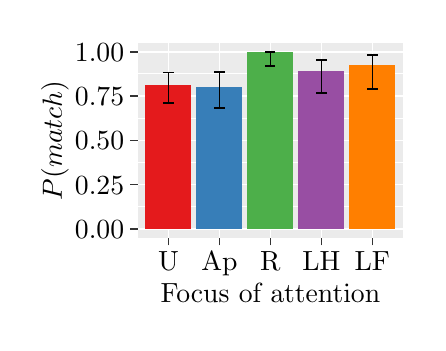
\begin{tikzpicture}[x=1pt,y=1pt]
\definecolor{fillColor}{RGB}{255,255,255}
\path[use as bounding box,fill=fillColor,fill opacity=0.00] (0,0) rectangle (141.12,106.79);
\begin{scope}
\path[clip] (  0.00,  0.00) rectangle (141.12,106.79);
\definecolor{drawColor}{RGB}{255,255,255}
\definecolor{fillColor}{RGB}{255,255,255}

\path[draw=drawColor,line width= 0.6pt,line join=round,line cap=round,fill=fillColor] ( -0.00,  0.00) rectangle (141.12,106.79);
\end{scope}
\begin{scope}
\path[clip] ( 39.80, 30.86) rectangle (135.62,101.29);
\definecolor{fillColor}{gray}{0.92}

\path[fill=fillColor] ( 39.80, 30.86) rectangle (135.62,101.29);
\definecolor{drawColor}{RGB}{255,255,255}

\path[draw=drawColor,line width= 0.3pt,line join=round] ( 39.80, 42.07) --
	(135.62, 42.07);

\path[draw=drawColor,line width= 0.3pt,line join=round] ( 39.80, 58.07) --
	(135.62, 58.07);

\path[draw=drawColor,line width= 0.3pt,line join=round] ( 39.80, 74.08) --
	(135.62, 74.08);

\path[draw=drawColor,line width= 0.3pt,line join=round] ( 39.80, 90.09) --
	(135.62, 90.09);

\path[draw=drawColor,line width= 0.6pt,line join=round] ( 39.80, 34.06) --
	(135.62, 34.06);

\path[draw=drawColor,line width= 0.6pt,line join=round] ( 39.80, 50.07) --
	(135.62, 50.07);

\path[draw=drawColor,line width= 0.6pt,line join=round] ( 39.80, 66.08) --
	(135.62, 66.08);

\path[draw=drawColor,line width= 0.6pt,line join=round] ( 39.80, 82.08) --
	(135.62, 82.08);

\path[draw=drawColor,line width= 0.6pt,line join=round] ( 39.80, 98.09) --
	(135.62, 98.09);

\path[draw=drawColor,line width= 0.6pt,line join=round] ( 50.86, 30.86) --
	( 50.86,101.29);

\path[draw=drawColor,line width= 0.6pt,line join=round] ( 69.29, 30.86) --
	( 69.29,101.29);

\path[draw=drawColor,line width= 0.6pt,line join=round] ( 87.71, 30.86) --
	( 87.71,101.29);

\path[draw=drawColor,line width= 0.6pt,line join=round] (106.14, 30.86) --
	(106.14,101.29);

\path[draw=drawColor,line width= 0.6pt,line join=round] (124.56, 30.86) --
	(124.56,101.29);
\definecolor{fillColor}{RGB}{228,26,28}

\path[fill=fillColor] ( 42.57, 34.06) rectangle ( 59.15, 86.00);
\definecolor{fillColor}{RGB}{55,126,184}

\path[fill=fillColor] ( 60.99, 34.06) rectangle ( 77.58, 85.48);
\definecolor{fillColor}{RGB}{77,175,74}

\path[fill=fillColor] ( 79.42, 34.06) rectangle ( 96.00, 98.09);
\definecolor{fillColor}{RGB}{152,78,163}

\path[fill=fillColor] ( 97.85, 34.06) rectangle (114.43, 90.98);
\definecolor{fillColor}{RGB}{255,127,0}

\path[fill=fillColor] (116.27, 34.06) rectangle (132.86, 93.40);
\definecolor{drawColor}{RGB}{0,0,0}

\path[draw=drawColor,line width= 0.6pt,line join=round] ( 49.02, 90.60) --
	( 52.70, 90.60);

\path[draw=drawColor,line width= 0.6pt,line join=round] ( 50.86, 90.60) --
	( 50.86, 79.65);

\path[draw=drawColor,line width= 0.6pt,line join=round] ( 49.02, 79.65) --
	( 52.70, 79.65);

\path[draw=drawColor,line width= 0.6pt,line join=round] ( 67.44, 90.85) --
	( 71.13, 90.85);

\path[draw=drawColor,line width= 0.6pt,line join=round] ( 69.29, 90.85) --
	( 69.29, 77.81);

\path[draw=drawColor,line width= 0.6pt,line join=round] ( 67.44, 77.81) --
	( 71.13, 77.81);

\path[draw=drawColor,line width= 0.6pt,line join=round] ( 85.87, 98.09) --
	( 89.55, 98.09);

\path[draw=drawColor,line width= 0.6pt,line join=round] ( 87.71, 98.09) --
	( 87.71, 92.97);

\path[draw=drawColor,line width= 0.6pt,line join=round] ( 85.87, 92.97) --
	( 89.55, 92.97);

\path[draw=drawColor,line width= 0.6pt,line join=round] (104.30, 95.14) --
	(107.98, 95.14);

\path[draw=drawColor,line width= 0.6pt,line join=round] (106.14, 95.14) --
	(106.14, 83.16);

\path[draw=drawColor,line width= 0.6pt,line join=round] (104.30, 83.16) --
	(107.98, 83.16);

\path[draw=drawColor,line width= 0.6pt,line join=round] (122.72, 96.87) --
	(126.41, 96.87);

\path[draw=drawColor,line width= 0.6pt,line join=round] (124.56, 96.87) --
	(124.56, 84.64);

\path[draw=drawColor,line width= 0.6pt,line join=round] (122.72, 84.64) --
	(126.41, 84.64);
\end{scope}
\begin{scope}
\path[clip] (  0.00,  0.00) rectangle (141.12,106.79);
\definecolor{drawColor}{RGB}{0,0,0}

\node[text=drawColor,anchor=base east,inner sep=0pt, outer sep=0pt, scale=  1.00] at ( 34.85, 30.62) {0.00};

\node[text=drawColor,anchor=base east,inner sep=0pt, outer sep=0pt, scale=  1.00] at ( 34.85, 46.63) {0.25};

\node[text=drawColor,anchor=base east,inner sep=0pt, outer sep=0pt, scale=  1.00] at ( 34.85, 62.63) {0.50};

\node[text=drawColor,anchor=base east,inner sep=0pt, outer sep=0pt, scale=  1.00] at ( 34.85, 78.64) {0.75};

\node[text=drawColor,anchor=base east,inner sep=0pt, outer sep=0pt, scale=  1.00] at ( 34.85, 94.65) {1.00};
\end{scope}
\begin{scope}
\path[clip] (  0.00,  0.00) rectangle (141.12,106.79);
\definecolor{drawColor}{gray}{0.20}

\path[draw=drawColor,line width= 0.6pt,line join=round] ( 37.05, 34.06) --
	( 39.80, 34.06);

\path[draw=drawColor,line width= 0.6pt,line join=round] ( 37.05, 50.07) --
	( 39.80, 50.07);

\path[draw=drawColor,line width= 0.6pt,line join=round] ( 37.05, 66.08) --
	( 39.80, 66.08);

\path[draw=drawColor,line width= 0.6pt,line join=round] ( 37.05, 82.08) --
	( 39.80, 82.08);

\path[draw=drawColor,line width= 0.6pt,line join=round] ( 37.05, 98.09) --
	( 39.80, 98.09);
\end{scope}
\begin{scope}
\path[clip] (  0.00,  0.00) rectangle (141.12,106.79);
\definecolor{drawColor}{gray}{0.20}

\path[draw=drawColor,line width= 0.6pt,line join=round] ( 50.86, 28.11) --
	( 50.86, 30.86);

\path[draw=drawColor,line width= 0.6pt,line join=round] ( 69.29, 28.11) --
	( 69.29, 30.86);

\path[draw=drawColor,line width= 0.6pt,line join=round] ( 87.71, 28.11) --
	( 87.71, 30.86);

\path[draw=drawColor,line width= 0.6pt,line join=round] (106.14, 28.11) --
	(106.14, 30.86);

\path[draw=drawColor,line width= 0.6pt,line join=round] (124.56, 28.11) --
	(124.56, 30.86);
\end{scope}
\begin{scope}
\path[clip] (  0.00,  0.00) rectangle (141.12,106.79);
\definecolor{drawColor}{RGB}{0,0,0}

\node[text=drawColor,anchor=base,inner sep=0pt, outer sep=0pt, scale=  1.00] at ( 50.86, 19.03) {U};

\node[text=drawColor,anchor=base,inner sep=0pt, outer sep=0pt, scale=  1.00] at ( 69.29, 19.03) {Ap};

\node[text=drawColor,anchor=base,inner sep=0pt, outer sep=0pt, scale=  1.00] at ( 87.71, 19.03) {R};

\node[text=drawColor,anchor=base,inner sep=0pt, outer sep=0pt, scale=  1.00] at (106.14, 19.03) {LH};

\node[text=drawColor,anchor=base,inner sep=0pt, outer sep=0pt, scale=  1.00] at (124.56, 19.03) {LF};
\end{scope}
\begin{scope}
\path[clip] (  0.00,  0.00) rectangle (141.12,106.79);
\definecolor{drawColor}{RGB}{0,0,0}

\node[text=drawColor,anchor=base,inner sep=0pt, outer sep=0pt, scale=  1.00] at ( 87.71,  7.44) {Focus of attention};
\end{scope}
\begin{scope}
\path[clip] (  0.00,  0.00) rectangle (141.12,106.79);
\definecolor{drawColor}{RGB}{0,0,0}

\node[text=drawColor,rotate= 90.00,anchor=base,inner sep=0pt, outer sep=0pt, scale=  1.00] at ( 12.39, 66.08) {\(P(match)\)};
\end{scope}
\end{tikzpicture}
